%%%%%%%%%%%%%%%%%%%%%%%%%%%%%%%%%%%%%%%%%%%%%%%%%%%%%%%%%%%%%%%%%%%%%%%%%%
%
%    phase1-GO.tex  (use only for General Observer and Snapshot proposals; use phase1-AR.tex for Archival Research and
%                      Theory proposals use phase1-DD.tex for GO/DD proposals and use phase1-MC.tex for GO/MC rapid response
%                       proposals).
%
%    HUBBLE SPACE TELESCOPE
%    PHASE I OBSERVING PROPOSAL TEMPLATE 
%     FOR CYCLE 25 and beyond
%
%    Version 2.1; November 2018
%
%    Guidelines and assistance
%    =========================
%     Cycle 27 Announcement Web Page:
%
%         https://hst-docs.stsci.edu/ 
%
%    Please contact the STScI Help Desk if you need assistance with any
%    aspect of proposing for and using HST. Either send e-mail to
%    help@stsci.edu, or call 1-800-544-8125; from outside the United
%    States, call [1] 410-338-1082.
%
%
%%%%%%%%%%%%%%%%%%%%%%%%%%%%%%%%%%%%%%%%%%%%%%%%%%%%%%%%%%%%%%%%%%%%%%%%%%%

% The template begins here. Please do not modify the font size from 12 point.

\documentclass[12pt]{article}
\usepackage{phase1}
\usepackage{graphicx}
\usepackage{natbib}
\usepackage{graphicx}
%\usepackage{sidecap}
\DeclareRobustCommand{\ion}[2]{%
\relax\ifmmode
\ifx\testbx\f@series
{\mathbf{#1\,\mathsc{#2}}}\else
{\mathrm{#1\,\mathsc{#2}}}\fi
\else\textup{#1\,{\mdseries\textsc{#2}}}%
\fi}


\def\aj{AJ}%

          % Astronomical Journal

\def\araa{ARA\&A}%

          % Annual Review of Astron and Astrophys

\def\apj{ApJ}%

          % Astrophysical Journal

\def\apjl{ApJ}%

          % Astrophysical Journal, Letters

\def\apjs{ApJS}%

          % Astrophysical Journal, Supplement

\def\ao{Appl.~Opt.}%

          % Applied Optics

\def\apss{Ap\&SS}%

          % Astrophysics and Space Science

\def\aap{A\&A}%

          % Astronomy and Astrophysics

\def\aapr{A\&A~Rev.}%

          % Astronomy and Astrophysics Reviews

\def\aaps{A\&AS}%

          % Astronomy and Astrophysics, Supplement

\def\azh{AZh}%

          % Astronomicheskii Zhurnal

\def\baas{BAAS}%

          % Bulletin of the AAS

\def\jrasc{JRASC}%

          % Journal of the RAS of Canada

\def\memras{MmRAS}%

          % Memoirs of the RAS

\def\mnras{MNRAS}%

          % Monthly Notices of the RAS

\def\pra{Phys.~Rev.~A}%

          % Physical Review A: General Physics

\def\prb{Phys.~Rev.~B}%

          % Physical Review B: Solid State

\def\prc{Phys.~Rev.~C}%

          % Physical Review C

\def\prd{Phys.~Rev.~D}%

          % Physical Review D

\def\pre{Phys.~Rev.~E}%

          % Physical Review E

\def\prl{Phys.~Rev.~Lett.}%

          % Physical Review Letters

\def\pasp{PASP}%

          % Publications of the ASP

\def\pasj{PASJ}%

          % Publications of the ASJ

\def\qjras{QJRAS}%

          % Quarterly Journal of the RAS

\def\skytel{S\&T}%

          % Sky and Telescope

\def\solphys{Sol.~Phys.}%

          % Solar Physics

\def\sovast{Soviet~Ast.}%

          % Soviet Astronomy

\def\ssr{Space~Sci.~Rev.}%

          % Space Science Reviews

\def\zap{ZAp}%

          % Zeitschrift fuer Astrophysik

\def\nat{Nature}%

          % Nature

\def\iaucirc{IAU~Circ.}%

          % IAU Cirulars

\def\aplett{Astrophys.~Lett.}%

          % Astrophysics Letters

\def\apspr{Astrophys.~Space~Phys.~Res.}%

          % Astrophysics Space Physics Research

\def\bain{Bull.~Astron.~Inst.~Netherlands}%

          % Bulletin Astronomical Institute of the Netherlands

\def\fcp{Fund.~Cosmic~Phys.}%

          % Fundamental Cosmic Physics

\def\gca{Geochim.~Cosmochim.~Acta}%

          % Geochimica Cosmochimica Acta

\def\grl{Geophys.~Res.~Lett.}%

          % Geophysics Research Letters

\def\jcp{J.~Chem.~Phys.}%

          % Journal of Chemical Physics

\def\jgr{J.~Geophys.~Res.}%

          % Journal of Geophysics Research

\def\jqsrt{J.~Quant.~Spec.~Radiat.~Transf.}%

          % Journal of Quantitiative Spectroscopy and Radiative Trasfer

\def\memsai{Mem.~Soc.~Astron.~Italiana}%

          % Mem. Societa Astronomica Italiana

\def\nphysa{Nucl.~Phys.~A}%

          % Nuclear Physics A

\def\physrep{Phys.~Rep.}%

          % Physics Reports

\def\physscr{Phys.~Scr}%

          % Physica Scripta

\def\planss{Planet.~Space~Sci.}%

          % Planetary Space Science

\def\procspie{Proc.~SPIE}%

          % Proceedings of the SPIE

\let\astap=\aap

\let\apjlett=\apjl

\let\apjsupp=\apjs

\let\applopt=\ao

%

\uchyph=0

%\bibpunct{(}{)}{;}{a}{}{,}

\begin{document}

%   1. SCIENTIFIC JUSTIFICATION
%       (See https://hst-docs.stsci.edu/display/HSP/HST+Cycle+27+Preparation+of+the+PDF+Attachment)
%
%
\justification          % Do not delete this command.
% Enter your scientific justification here. 
Stars and planetary systems continue to form in our Milky Way today. High resolution imaging of star-forming regions provides unique information on the rich phenomenology that characterizes these regions and has produced some of the most spectacular images ever taken by
the Hubble Space Telescope (HST, e.g.\ Fig.~\ref{fig:reiter}).
When cloud fragments start to collapse into protostars, they are still deeply
embedded in a dusty envelope and can be only seen in the sub-mm and far-IR (class
0 sources). Because angular momentum is conserved, infall does not happen
radially all the way down, but instead an accretion disks takes shape while
the remaining envelope still hides the inner core from view in all but the
mid/far-IR (class I sources).  These young objects also often drive powerful jets
that propagate through the envelope and pierce the cloud. Once the envelope
dissipates, the stars become visible in the optical  (class II sources), while dust grains in the accreting disks start to coagulate
into planets. Once the disks deplete due to planet formation, accretion or
evaporation, planetary system remains around a young, active star
(class III sources). For late-type stars, this evolutionary process takes several Myrs,
while massive stars can go through a similar sequence much faster, meaning that
they are typically still surrounded by dense cloud material when they reach the main-sequence.
The unresolved central objects can be studied from the spectral energy distribution, but
high-resolution imaging from facilities like e.g. ALMA and -in this case- HST  is critical to understand how disks, jets, and the remaining envelope
appear like, evolve and interact each other (see Fig.~\ref{fig:krist}, \ref{fig:reiter},  \ref{fig:ONCACS}).


\begin{figure}
    \centering
    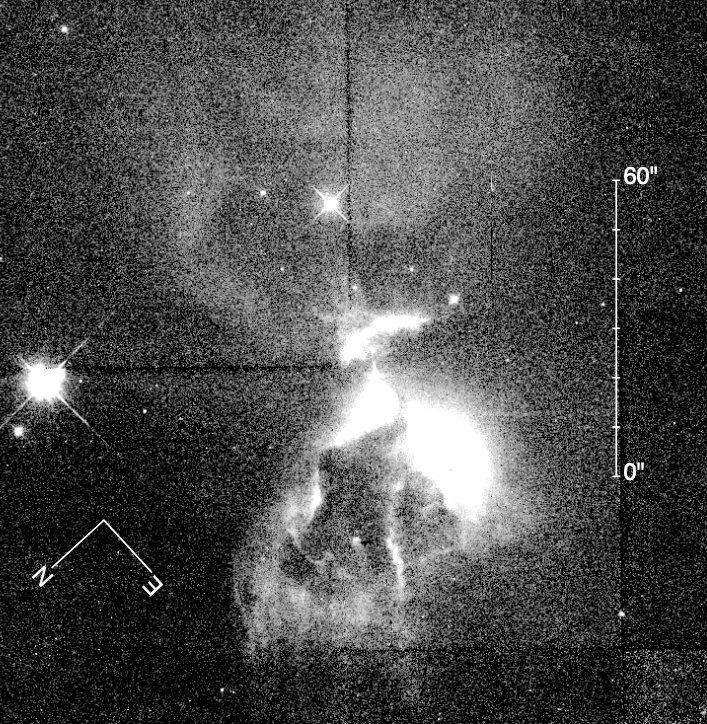
\includegraphics[height=8cm]{Krist98.png}
    \caption{Young, low-mass star FS Tauri in low-mass star-forming region observed with WFPC2. The image is combined from several exposures mostly in the F675W filter. Average exposure time is about 800~s. The image reveals an hour-glass shaped reflection nebula and a jet. From: \citet{1998ApJ...501..841K}.}
    \label{fig:krist}
\end{figure}




\begin{figure}
    \centering
    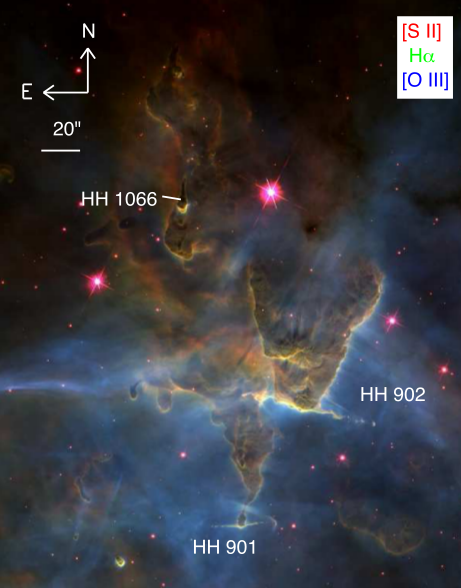
\includegraphics[width=.45\textwidth]{reiter13_fig3.png}
    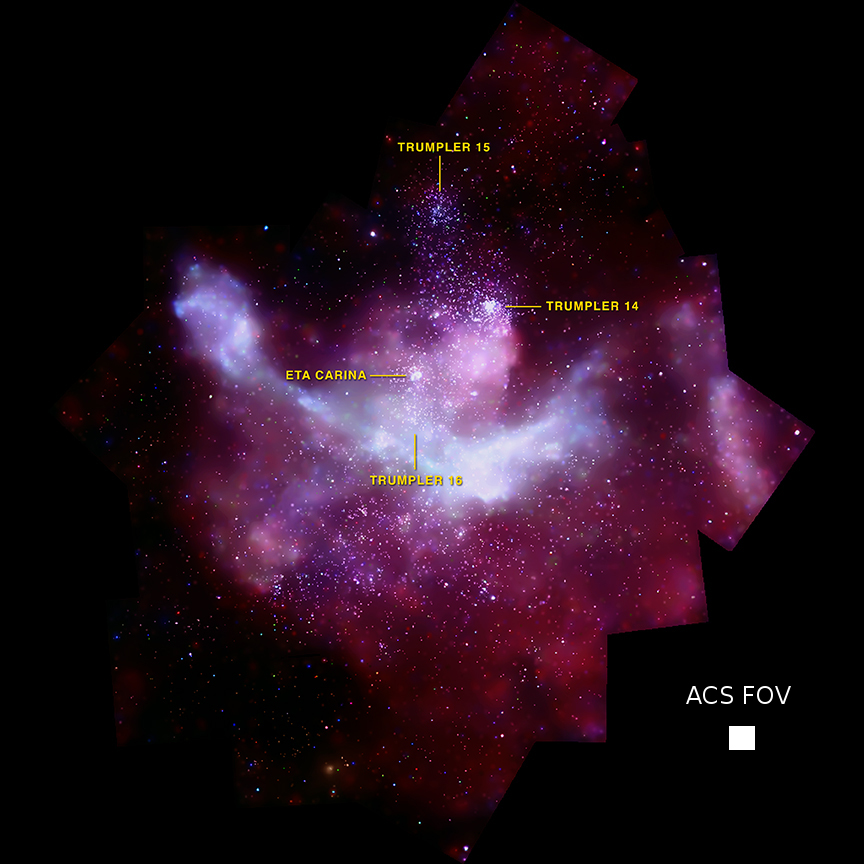
\includegraphics[width=.54\textwidth]{carina_xray_label.jpg}
    \caption{\emph{Left:} Protostellar jets in the Carina region, observed with WFC3 in same filters we propose to use; exposure time about 2000~s for H$\alpha$ and about 3000~s for [O~{\sc iii}]. From: \citet{2013MNRAS.433.2226R} \emph{Right:} X-ray view of the entire Carina star-forming region. This image is about 1 degree across and shows that practically any location for a WFC3 or ACS pointing in the star-forming region will show young stars with disks (Chandra discovered $> 14,000$ source) and ionized plasma. The white box in the bottom right shows the approximate field-of-view (FOV) of ACS or WFC3. Image credit: NASA/CXC/PSU/L.Townsley et al.}
    \label{fig:reiter}
\end{figure}

\section{Surveys of star-forming regions}
The Chandra X-ray observatory has surveyed with sub-arsecond spatial resolution  many of the massive star-forming regions in the Milky Way
in X-rays (e.g.\ \citealt{2011ApJS..194....1T} for Carina,
\citealt{2010ApJ...713..871W} for Cyg OB2, \citealt{2005ApJS..160..379F} for
the Orion Nebula Cloud, \citealt{2008AJ....135..693W} for RCW 108) and 
%a surprising number of the 
several lower-mass star-forming regions
(e.g.\ \citealt{2018AJ....155..241W} for Serpens, \citealt{2012AJ....144..101G}
for IRAS 20050+2720), but sub-arcsecond, wide-field surveys in the optical are rare.
In the IR, essentially
all star-forming regions have been observed with \emph{Spitzer} with a resolution between 1 and 2 arcsec
(e.g.\ \citealt{2009ApJS..184...18G} surveyed all star-forming regions within 1
kpc, and \citealt{2015ApJS..220...11D} the Gould Belt). Both IR and the hard
X-rays are less extincted than optical wavelength, and thus allow a
deeper view into the embedded regions. The combination of X-rays and IR information
is a great tool to identify the point sources in clusters and to establish
cluster membership. From the IR spectral energy distribution (SED) of a source one can
infer the presence of an accretion disk, especially when the IR excess can be measured over the stellar SED \citep{2009ApJS..184...18G}. However, \emph{Spitzer} and ground-based wide-field surveys typically only resolved the widest binaries (separated by arcseconds, or hundreds of au for near-by star-forming regions and thousands of au for further away high-mass star-forming regions).
%Essentially all young stars
%are active \citep{2018ApJS..235...43T}, and thus an X-ray detection is a good
%way to distinguish cluster members from older
%foreground stars \citep{2013ApJS..209...32B}. 

\section{Extended sources in star-forming regions}
Observations of star-forming regions reveal more than just point sources. The evolution of the
cloud as a whole, and therefore the star formation efficiency, the initial mass function, the possibility of triggering further generations of stars, depends on radiative and dynamical feedback from the forming stars, and thus the complex interplay between radiation, gas and dust in the turbulent environment (Fig.~\ref{fig:krist}). Probing these phenonmena requires different techniques. The
cool material below a few hundred K is visible in the radio as dust continuum
emission or in molecular gas emission lines; slightly warmer dust can be seen in
the IR. However, there are many processes that heat material above the dust
sublimation temperature and can therefore optimally be traced at visible wavelengths. 
They are among the most interesting ones in star-forming regions:
Irradiation by hot and bright massive stars, disk evaporation, stellar winds,
jet emission and shock fronts in the cloud material. Only the most energetic
processes (supernova explosions, O star winds) reach temperatures that can be seen as a faint
X-ray continuum emission (Fig.~\ref{fig:reiter}, right). The weak signal means that generally they 
cannot be studied at high spatial resolution.

Radio observations are also well-suited to survey large regions on the sky and to
trace wide-angle molecular outflows \citep[e.g.][]{2003MNRAS.341..707C} but
they miss the faster, more collimated and energetic outflow components which, according to \citep{2003ApJ...590L.107A}, originate
deeper in the gravitational potential, i.e.\ closer to the proto-star.


\section{Immediate objectives}
We propose a serendipitous, pure-parallel imaging survey of star-forming regions in the Milky Way utilizing the superb PSF and photometric stability of the WFC3 and ACS/WFC. The survey will use a combination of broad-band and narrow-band filters and some of the resulting images may be well suited to feature HST in the public.
Scientifically, such a survey can contribute to any study using SEDs of point sources or looking at resolved structure, but the following science questions will be addressed in detail.

\begin{figure}
    \centering
    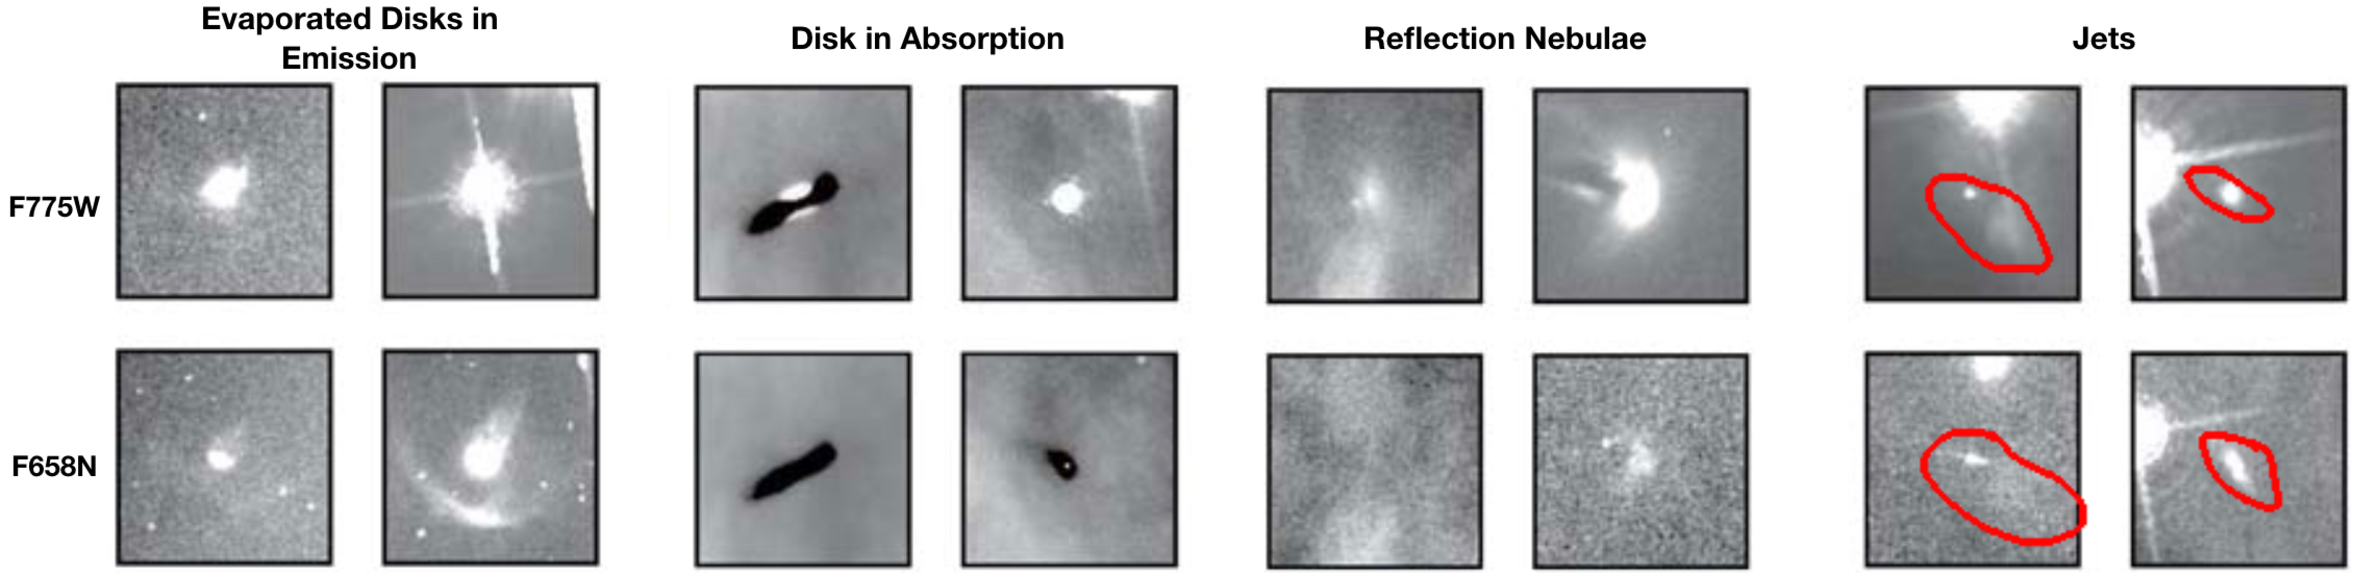
\includegraphics[width=\textwidth]{hst_disks_v4.pdf}
    \caption{Examples of different objects detected in an ACS survey of the Orion Nebula Cloud by \citet{2008AJ....136.2136R}, each column shows one object in two different filters (\emph{top}: F775W = SDSS $i'$, \emph{bottom}: F658N = H$\alpha$). For each category, two objects are shown. Note how some features stand out better in the emission line, while others are visible in the broad-band.}
    \label{fig:ONCACS}
\end{figure}

\subsection{Jet sources and jet launching}
It is unknown how jets are launched and collimated, but ultimately, they have
to be powered by the gravitational energy released during the accretion process. In
nearby stars, jets are layered like an onion where slower, outer layers are
surrounded by hotter and faster layers inside \citep{1993ApJ...409..748G,2000ApJ...537L..49B}. The
innermost layers can reach a few 1000~km/s for jets from massive stars and heat
up to X-ray emitting temperatures, but the bulk of the mass is neutral or
moderately ionized and emits H$\alpha$, or optical emission lines such as
[O~{\sc i}] 6300\AA{} or [O~{\sc iii}] 5007\AA{} (Fig.~\ref{fig:reiter},
left or Fig.~\ref{fig:ONCACS}, rightmost sources). The sample of well-studied jets is surprisingly small, especially for
later stages of star formation and lower mass sources where jets are less
powerful and thus fainter and harder to find. Such micro-jets are sometimes
only a few arcseconds long, with the brightest part of the emission close to
the star and provide crucial information on the collimation mechanism. From the ground, those jets can only be seen with adaptive optics
imaging and will not be found in large-scale surveys but they are easily
visible in HST images. Even for more powerful jets, which are resolved at
resolutions typical for ground-based seeing, we often require high-resolution
imaging to identify the jet source or to image their internal structure.


\subsection{Knots in jets}
Jets are not homogeneous but show knots, internal working surfaces, and termination shocks (Fig.~\ref{fig:reiter}, left). These can be due to mass-ejection events in the past, and, since mass ejection and accretion are related, contain a fossil archive of previous accretion rates \citep{2014A&A...563A..87E}. As knots move away from the source, they become fainter. If jet emission switches on an off in a source, there may be no indication of a jet seen in the star today; thus surveys looking for jets would not target those sources, however, fossil records of previous jet event may still be out there in the form of faint emission regions, at some distance from the source. HST imaging in a blind search in H$\alpha$ and [O~{\sc i}] is a promising way to find those features. This is actually easier in low-mass star-forming regions where the source density is lower and thus the likely jet source can be identified, even if emission is not seen close to it.

\subsection{Disk evolution and evaporation}


Theoretically, we expect that the lifetimes of disks depend strongly on the formation environment, where massive stars in dense clusters should evaporate disks within a Myrs or so and close encounters can strip additional material from the disks \citep[e.g.][]{2004ApJ...611..360A,2019MNRAS.485.1489W,2019arXiv190211094N} but there are recent indications that external photo-evaporation can be important even in low-mass star-forming regions \citep{2017MNRAS.468L.108H}.
There are two ways to study this observationally: Look how disk properties in a massive cluster change with distance from the most massive members \citep{2014ApJ...784...82M,2017AJ....153..240A,2018ApJ...860...77E}, or compare clusters of different mass. Our proposed study can help with both (see disks in absorption and evaporating disks in Fig.~\ref{fig:ONCACS} for examples how this might look), giving us high-resolution observations of low-mass star-forming regions where normally one would not invest much time on a blind survey to find disks in imaging, and images of massive clusters, a little further away from the objects usually studied. Extinction measurements will also provide a 3-D view of the matter distribution on the front edge of the cloud, enabling a more accurate determination of the actual photon flux irradiating the disks. 
Understanding external photoevaporation is also important for the history of the solar systems and the formation of our Earth \citep{2015ApJ...815..112K}.

\subsection{Multiplicity}
A large fraction of all young stars forms in binaries or higher order multiples, yet many questions about the evolution of multiple systems remain unsolved. First, simply knowing the fraction of multiple systems and the mass and radius distribution of companions can tell us under what conditions companions grow in the disk of the primary (like planets) versus how the envelope forms two stars. If we can image disks or outflows of at least one of the stars, we can also start to probe if the orbital plane and individual disks are aligned.

For close-in binaries, the companion will obviously change the evolution of the primary's disk, e.g. by triggering episodic accretion \citep{2013ApJ...766...62G}, and thus possibly reducing the time and the mass reservoir available for planet formation. For binaries with separations comparable to the size of a disk in the T Tauri phase (a few hundred au) this is less clear. In the well-studied case of RW~Aur~A and B a tidal stream connects the disks \citep{2006A&A...452..897C}. However, to study these effects in a sample, we first need an accurate census of multiplicity and how this might change with the mass of the central star and its formation environment.

For all these reasons, we need to identify more systems with companions. One of
the best methods to do that is space-based imaging in $R$, $I$, or the near-IR where the contrast between the primary and a lower mass secondary is less extreme than in, e.g.\ the $V$ band. 

\citet{2001A&A...379..147D} find that about 20\% of their sample in the young
cluster NGC 6611 have a companion in the range 200-3000~au, where the companion
has at least a tenth of the mass of the primary. With HST's sub-arcsecond PSF,
we can detect a K8 companion at 200~au distance from a moderately bright
primary for star-forming regions at 1 kpc, and we can perform reliable photometry on companions separated by approximately 500~au. 


\section{High-resolution images without a primary orbit cost}
We propose a pure-parallel survey in the optical with \emph{HST}. In a pure
parallel observation, we do not specify individual targets, but simply switch
on the WFC3 or ACS cameras when \emph{HST} is observing any target in a star
forming region with STIS or COS; we will see essentially random fields a few
arcminutes away from the primary spectroscopic target. Thanks to ULYSSES, an
initiative using 500-1000 orbits of director's time for UV spectroscopy of
young stars over the next three years, we know that a large number of orbits
will be allocated to spectroscopic targets in star-forming regions in addition
to what the TAC recommends. \emph{This is an unprecedented opportunity to allocate a significant number of orbits to a deep and wide survey of serendipitous features in star-forming regions; in other cycles, there are simply not enough primary orbits available to schedule a parallel program long enough to sample significant area.}

For the primary
\emph{HST} observations, observers often choose ``special'' locations,
e.g.\ the brightest and most active stars in a star-forming region. A census
measuring the effect of photoevaporation in these regions does not necessarily
represent the typical state of star formation; in fact, any concentration of
observations in the center of a star-forming region (where the highest number
of sources is found) biases a study towards effects of dense
environments. While our pointings will not be truly randomly distributed, they
will cover a range of star-forming environments in different clusters that has
not been studied with such high spatial resolution and such uniform filter
coverage before. A true blind survey of large areas of star-forming regions is prohibitively expensive; on the other hand, a pure-parallel survey like we suggest costs no primary orbits and also avoids sampling bias to a large degree.

Pure-parallel surveys have taken deep images in star-forming regions before and
have been used for extragalactic astronomy \citep{2007A&A...468..823S} but also
to search for galactic ultracool objects such as L and T dwarfs
\citep{2005ApJ...631L.159R}. These studies show the potential for serendipitous
science from the deep high-resolution imaging proposed here. We analyzed some of this archival data and verified that structures of the
molecular cloud are indeed visible in great detail; however, all those data are
taken in wide filters only while we propose additional observations in narrow
band filters which probe particular conditions in irradiated clouds, disks and
jets.


\section{Estimating the yield of the proposed survey}
Our proposed observing strategy is very similar to the atlas of protoplanetary disks in the Orion Nebula \citep{2008AJ....136.2136R,2013ApJS..207...10R}. Their survey covers about 450~arcmin$^2$ in $B$, $V$, H$\alpha$, $I$, and $z$ with average exposure times of about 400~s. They detect about 3200 compact sources and 219 sources with circumstellar matter. The largest fraction of those (178) are externally ionized disk in emission; 36 disks are seen in extinction against the bright nebula in the background. Five objects show jets without an apparent disk (meaning that the disk is likely to be smaller because the objects are more evolved). Figure~\ref{fig:ONCACS} shows examples of these detections. 

In a request for 100 pure-parallel obits we will sample about 0.3 sq deg of
area in several star-forming clouds, likely including both nearby low-mass
star-forming regions and higher-mass star-forming regions at a larger distance.
%This is several orders of magnitude less than the large \emph{Spitzer} surveys
%of star-forming regions, but it will still be the largest dataset available
%with the superb spatial resolution that HST offers and the number of filters we
%plan to use.
 Ground-based based surveys are typically only done in broad-band
filters \citep[IPHAS, which also includes an H$\alpha$ filter is an
  exception][]{2005MNRAS.362..753D} and without adaptive optics, thus the
space-based \emph{HST} images that we will obtain will be superior in spatial
resolution, depth, and coverage of spectral features.


Depending on the star-forming region where the primary targets are located, the
number of objects we can detect will differ. If the primary targets are in
dense star-forming regions such as the Orion Nebula Cloud or Carina, we are
virtually guaranteed to see several young stars, cloud structures, disks and
outflows for any target location; on the other hand, if the primary targets are
in close-by low-density star-forming regions such as Taurus, we may find some
fields devoid of cluster members, but probing regions usually ignored in current surveys. 




%%%%%%%%%%%%%%%%%%%%%%%%%%%%%%%%%%%%%%%%%%%%%%%%%%%%%%%%%%%%%%%%%%%%%%%%%%%

%   2. DESCRIPTION OF THE OBSERVATIONS
%       (See https://hst-docs.stsci.edu/display/HSP/HST+Cycle+27+Preparation+of+the+PDF+Attachment)
%
%
\describeobservations   % Do not delete this command.
% Enter your observing description here.
For pure-parallel programs such as ours, STScI will prepare lists of primary orbits, which may be suitable for the execution of the parallel observations. Since we will have no influence over the setup of those spectroscopic observations, the exact pointing, orientation and number of dither positions will be determined by the primary science program. Thus, we can only describe a general set-up of the observations, under the assumptions that the details will have to be adjusted in Phase II.

Broad-band images will allow us to determine the SED of objects that may show IR excess with \emph{Spitzer} or X-ray activity with Chandra, allowing us to firmly identify and preliminary characterize a substantial number of pre-main-sequence objects. For objects that turn out to be single in our observations, we can combine the data in the two or three broad bands that we take with observations from all-sky surveys, such as GAIA. Even if we resolve a binary system, combining our resolved fluxes with unresolved photometry and additional information, such as the parallax (from GAIA), we can constrain masses and extinction for both components.

Narrow band images trace instead the rich phenomenology typical of these regions. In particular, in 
high-mass star-forming regions, [O~{\sc iii}] is a good tracer of hot nebular gas, either radiatively or collisionally excited, whereas in low-mass star-forming regions, [O~{\sc iii}] 5007\AA{} only traces shock excitation (jets and HH objects). The soft-UV flux typical of these regions supports the complex chemical networks typical of PDR regions, which includes [O~{\sc i}] emission from the photodissociation of water molecules. WFC3 has a larger choice of narrow-band filters, and, if we have the opportunity (see below) we propose to add observations in [O~{\sc i}] 6300\AA{} and two lines in the UV that are unique to \emph{HST}/WFC3 because they are inaccessible from the ground (Mg~{\sc ii} 2800\AA{} and [Ne~{\sc v}] 3426\AA{}) as well as additional broad-band WFC2 $V$ images. In particular, Mg~{\sc ii} 2800\AA{} has been shown to be strong, even stronger than H$\alpha$ in jets from low-mass stars \citep{2007ApJ...663..350C}.

 Table~\ref{tab:setup} summarizes the filters to be used.
For a typical usable orbit time of about 2800~s after acquisition, we can take exposures of different depth in the most suitable filters, determined by the brightness of the stars (estimated using e.g.\ the GAIA database) and morphological complexity of the diffuse medium. If we schedule four exposures of about 540~s per orbit, the buffer dump can be done while the next exposure is in progress, thus our default setup in table~\ref{tab:setup} plans for four filters per orbit. 
Once we know the exact duration of the orbit (which depends on the position and roll angle specified by the primary target), we will optimize the exposure times considering also the overheads associated to buffer dumps and filter changes.


%\begin{table}[htbp]
%    \centering
%    \begin{tabular}{c|ccc}
%    \hline\hline
%           & WFC3 & WFC3 & ACS/WFC \\
%        star-forming region & high-mass & low-mass & any\\
%        \hline
%        SDSS $r'$ & F625W & F625W & F625W \\
%        SDSS $i'$ & F775W & F775W & F775W\\
%        H$\alpha$ & F656N & F656N & F658N\\{}
%        [O~{\sc iii}] 5007\AA{} & F502N & -- & F502N\\{}
%        [O~{\sc i}] 6300\AA{}& -- & F631N & -- \\
%        \hline
%    \end{tabular}
%    \caption{Filters to be used for observations in high and low-mass star-forming regions.}
%    \label{tab:setup}
%\end{table}

\begin{table}[htbp]
    \centering
    \begin{tabular}{c|ccc}
    \hline\hline
              & orbit 1, 4, 7, ... & orbit 2, 5, 8, ... & orbit 3, 6, 9, ... \\
              \hline
instrument    & WFC3 & ACS/WFC & WFC3 \\
\hline
bands/filters & SDSS $r'$ (F625W) & SDSS $r'$ (F625W) & 
               WFPC2 V (F555W)\\
              & SDSS $i'$ (F775W) & SDSS $i'$ (F775W) & 
              [Ne~{\sc v}] (F343N)\\
              & H$\alpha$ (F656N) & H$\alpha$ (F658N) & 
              Mg~{\sc ii} (F280N)\\
              & [O~{\sc iii}] (F502N) & [O~{\sc iii}]  (F502N) &
              [O~{\sc i}] (F631N)\\
        \hline
    \end{tabular}
    \caption{Default setup, using four filters per orbit. For each target position, we observe with the WFC3 first, then the ACS, then the WFC3 again. If we have more than three orbits per target position, we will cycle through the sequence again. The setup for each orbit will be adjusted depending on the time available per orbit and the brightness of known stars and morphological complexity of the medium as far as known.}
    \label{tab:setup}
\end{table}

If we have only one orbit with a specific pointing, we will perform imaging with the WFC3 because it is located closer to the STIS or COS FOV. In a star-forming region, a STIS or COS observation is most likely centered on a bright, active star and thus observing closer to it increases the chances to find irradiated cloud or outflow features. However,
it is typical for FUV spectroscopic observations to last for more than one orbit. In those cases, we may have access to more than one parallel orbit with almost the same pointing. We will use the extra orbits for additional observations with ACS/WFC and to observe in other filters in the WFC3 (see table~\ref{tab:setup}). ACS has a FOV a few arcmin away from WFC3. The ACS is equipped with fewer filters than the WFC3 and thus there would be little use to add another orbit for a second set of filters in the ACS.
In general, if we have more than three orbits with the same pointing, we plan to repeat the cycle of three orbits (WFC3, ACS, and WFC3 with other filters) observations to detect fainter features and to take advantage of multiple dither positions (if the primary observation dithers); taking multiple exposures in each filter will also mitigate against cosmic rays. 

We checked the HST archive for STIS and COS observations in star-forming regions as well as previous pure-parallel programs. It turns out that it is not uncommon to have 5-10 orbits with very similar pointings. This would give us a total exposure time of over a thousand seconds per filter. To achieve the longest integration times, HST may end up observing the primary spectroscopic targets at different roll angles. In this case, WFC3 and ACS will probe different areas on the sky, distributed over a circular corona centered on the primary target. Adding up the FOV for WFC and ACS and assuming on average 3-5 orbits with the same pointing, we estimate that with a request of 100 pure parallel orbits we will sample 300-400 sq.\ arcmin deg of star-forming regions.

\textbf{Sensitivity:} In a single orbit (exposure 540~s in each filter), we can detect an M7 star in a close star-forming region (130~pc) or an M2 at 0.5~kpc; sources like this should also be part of 2MASS, giving us fluxes in five colors so that we can fit the spectral type, extinction, and check for the presence of a disk in the spectral energy distribution \citep[SED, using models from][]{2007ApJS..169..328R}.
See the figures in the text above for examples of resolved cloud or jet emission features that were found in observations comparable to what we propose here.

Note that this is a request for a (mostly) blind survey. Since the targets of the primary observations are not known, we do not know what number of features we will find. Obviously, more observing time will allow us to cover a larger area or go deeper (depending on the distribution of targets for the primary observations). At the same time, this program is still useful if only a smaller number than the requested 100 orbits is granted or available; in this case we will simply survey a smaller area (or not as deep, depending on the distribution of primary targets).

\vspace{1mm}
\noindent The ULLYSES announcement encourages pure-parallel programs that can be executed in parallel to the Director's Discretionary Time spectroscopy and we are responding to that announcement here.


%%%%%%%%%%%%%%%%%%%%%%%%%%%%%%%%%%%%%%%%%%%%%%%%%%%%%%%%%%%%%%%%%%%%%%%%%%%

%   3. SPECIAL REQUIREMENTS
%       (See https://hst-docs.stsci.edu/display/HSP/HST+Cycle+27+Preparation+of+the+PDF+Attachment)
%
%
\specialreq             % Do not delete this command.
% Justify your special requirements here, if any.
None.

%%%%%%%%%%%%%%%%%%%%%%%%%%%%%%%%%%%%%%%%%%%%%%%%%%%%%%%%%%%%%%%%%%%%%%%%%%%

%   4. COORDINATED OBSERVATIONS
%       ((See https://hst-docs.stsci.edu/display/HSP/HST+Cycle+27+Preparation+of+the+PDF+Attachment)
%
%
\coordinatedobs          % Do not delete this command.
% Enter your coordinated observing plans here, if any.
None.

%%%%%%%%%%%%%%%%%%%%%%%%%%%%%%%%%%%%%%%%%%%%%%%%%%%%%%%%%%%%%%%%%%%%%%%%%%%

%   5. JUSTIFY DUPLICATIONS
%       (See https://hst-docs.stsci.edu/display/HSP/HST+Cycle+27+Preparation+of+the+PDF+Attachment)
%
%
\duplications           % Do not delete this command.
% Enter your duplication justifications here, if any.
If a region on the sky that would we available to this program has been observe before with these or similar filters, the new observations still add additional data to look for fainter objects and to study proper motion in the field (e.g.\ the expansion of a gas bubble or the motion of a know in a jet).

%%%%%%%%%%%%%%%%%%%%%%%%%%%%%%%%%%%%%%%%%%%%%%%%%%%%%%%%%%%%%%%%%%%%%%%%%%%
\bibliographystyle{aa} % style aa.bst
\bibliography{biblio}


\end{document}          % End of proposal. Do not delete this line.
                        % Everything after this command is ignored.
Title: A pure-parallel search for faint stuff in star-forming regions

Abstract
--------
star-forming regions contain many resolved structures, ranging from disks around individual stars, to narrow and wide binaries to large-scale outflows, bubbles and shock fronts traversing the entire cloud. In many cases, optical high-resolution imaging is the best tool to find and study these objects. We propose a pure-parallel survey, where no primary orbits are allocated and instead or observations are performed on whatever happens to be in the field-of-view of the WFC3 or ACS when other programs use STIS or COS on targets in star-forming regions. In this way, we can survey a large area to discover (i) previously unresolved companions, (ii) jets and outflows from young stars and (iii) irradiated and evaporating disks. Typically, such imaging studies are done in the most "interesting" regions close to the most massive and brightest stars. Our survey can complement that by imaging more "typical" parts of the cloud. We will use a combination of broad-band filters to detect nebulosity and identify and separate point sources as well as narrow-band filters in emission lines typically seen from irradiated disks, jets, and outflows.
